\documentclass[manuscript,screen,oneside]{acmart}

\usepackage{booktabs}
\usepackage{tabularx}
\usepackage{array}
\usepackage{graphicx}
\usepackage{tikz}
\usetikzlibrary{arrows.meta,positioning,shapes.geometric,fit,calc}

\setcopyright{none}
\settopmatter{printacmref=false}
\renewcommand{\footnotetextauthorsaddresses}[1]{}
\renewcommand{\footnotetextcopyrightpermission}[1]{}
\acmDOI{}
\acmISBN{}
\acmYear{2026}
\copyrightyear{2026}
\acmJournal{CSUR}

\title{Context-Window Degradation and Its Impact on Long-Document Research Synthesis}
% Author intentionally omitted for the submitted review-paper copy.

\begin{abstract}
Long-context large language models can accept inputs far longer than earlier language models, but a larger nominal context window does not guarantee reliable use of all information contained within it. This review synthesizes 20 scholarly papers identified through ResearchRabbit, Litmaps, Semantic Scholar, and Elicit. The literature is organized around four themes: context extension and capacity; empirical degradation and positional effects; evaluation and long-context reasoning; and mitigation through retrieval, efficient attention, training, and alignment. Across these themes, the evidence supports a distinction between nominal context capacity and effective context use. Performance can degrade as inputs grow, when relevant information is positioned unfavorably, when distractors accumulate, and when a task requires evidence to be integrated across distant locations. The review compares five approach families and identifies research gaps in realistic multi-document synthesis, source attribution, structure-aware evaluation, and adaptive selection between full-context inference and retrieval or compression. The central implication is that long-context capability should be evaluated as a task- and evidence-dependent reliability property rather than as a single maximum-token specification.
\end{abstract}

\keywords{long-context language models, context-window degradation, lost-in-the-middle, long-document synthesis, retrieval, long-context evaluation, positional bias, multi-document reasoning, context extension}

\ccsdesc[500]{Computing methodologies~Natural language processing}
\ccsdesc[500]{Information systems~Information retrieval}
\ccsdesc[300]{Computing methodologies~Knowledge representation and reasoning}

\DeclareCaptionFont{reviewcap}{\fontsize{10.5pt}{13pt}\selectfont}
\captionsetup{font=reviewcap,labelfont=bf}

\AtBeginDocument{%
  \fontsize{12pt}{15pt}\selectfont
  \renewcommand{\bibfont}{\fontsize{10.5pt}{13pt}\selectfont}%
}

\begin{document}
% Use identical margins on every page; no mirrored odd/even-page layout.
\setlength{\evensidemargin}{\oddsidemargin}
\setlength{\textwidth}{\dimexpr\paperwidth-1in-\oddsidemargin-\hoffset-\oddsidemargin-\hoffset\relax}
% Keep the body readable and consistent throughout the manuscript.
\renewcommand{\normalsize}{\fontsize{12pt}{15pt}\selectfont}
\renewcommand{\small}{\fontsize{11pt}{13.5pt}\selectfont}
\renewcommand{\footnotesize}{\fontsize{10.5pt}{13pt}\selectfont}
\maketitle
\pagestyle{empty}
\thispagestyle{empty}

\section{Introduction}\label{sec:introduction}
The growth of transformer-based language models has been accompanied by a rapid expansion of advertised context windows. The Transformer established self-attention as a central mechanism for sequence modelling, while later work explored ways to extend usable sequence length beyond the limits seen during training \cite{vaswani2017attention}. Yet practical long-context performance is not determined solely by whether a model accepts a large input. The important question is whether the model can retrieve, connect, reason over, and synthesize information distributed across that input.

This distinction matters directly for research synthesis. A literature-review task may require a model to locate evidence in several papers, connect findings across documents, distinguish relevant from distracting material, preserve methodological limitations, and produce a coherent conclusion. A model can have sufficient nominal context capacity while still underusing information in the middle of the input, losing performance as the context grows, or failing when evidence must be combined across distant locations. The reviewed literature therefore shifts the research question from ``How many tokens can the model accept?'' to ``How much of a long context can the model use reliably, for which tasks, and under what evidence distributions?''

This review makes three contributions. First, it synthesizes evidence connecting context extension to effective-use failures rather than treating context length as a sufficient capability measure. Second, it organizes the literature into a practical taxonomy covering capacity, degradation, evaluation, and mitigation, with implications for research synthesis. Third, it identifies gaps that matter specifically for academic literature review: distributed evidence, source attribution, document structure, distractor control, and adaptive context selection. Figure~\ref{fig:taxonomy} summarizes this organization, while Figure~\ref{fig:conceptual-framework} connects the major stages of the problem.

\section{Review Scope and Synthesis Approach}\label{sec:scope}
The review synthesizes 20 scholarly papers identified through ResearchRabbit, Litmaps, Semantic Scholar, and Elicit. The evidence set covers foundational context-extension work, empirical studies of long-context degradation, benchmark development, long-context reasoning, retrieval and compression, efficient attention, and long-context training or alignment. The synthesis is thematic rather than a formal systematic review: papers are grouped according to the failure mode or intervention they illuminate, and their implications for long-document research synthesis are compared across themes.

The review focuses on four questions: (1) how context capacity is extended; (2) how effective context use changes with length, position, distractors, and reasoning complexity; (3) how these effects are evaluated; and (4) which mitigation strategies address them. This scope is important because a benchmark result is not automatically equivalent to reliability in a real literature-review workflow. The evidence therefore distinguishes retrieval from downstream reasoning and distinguishes nominal capacity from effective use.

\section{Background and Conceptual Foundation}\label{sec:background}
The Transformer introduced self-attention as a mechanism for relating tokens within a sequence. Long-context research builds on this foundation by modifying positional representations, training procedures, memory mechanisms, or attention computation. Press et al. demonstrated that linear biases can help a model extrapolate to longer sequences than those used during training, while Chen et al. showed that positional interpolation can extend the context window of pretrained large language models \cite{press2022train,chen2023extending}. These approaches increase usable input length, but they do not by themselves establish that all positions in that input are equally accessible.

For long-document research synthesis, effective context use has at least four dimensions: retrieval of relevant evidence, robustness to evidence position, integration of evidence across documents, and faithful synthesis. A benchmark that tests only whether a single fact can be retrieved may therefore overestimate performance on realistic research tasks.

Figure~\ref{fig:conceptual-framework} summarizes the relationships discussed throughout the review: context-extension methods increase available capacity, evaluation studies expose effective-use failures, mitigation methods attempt to reduce those failures, and the final objective is reliable long-document research synthesis.

\clearpage
\begin{figure}[p]
\centering
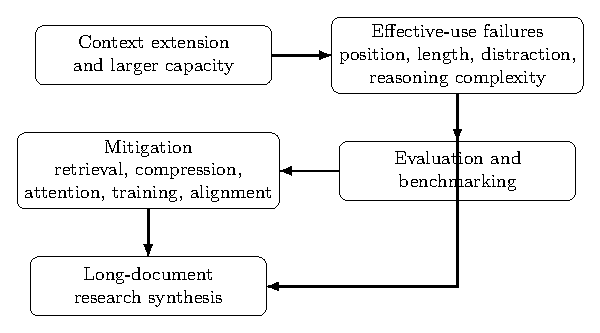
\includegraphics[width=.78\linewidth]{Figures/conceptual_framework.pdf}
\caption{Conceptual overview of the long-context research problem synthesized from the themes reviewed in this paper.}
\Description{A flow diagram linking context extension, effective-use failures, evaluation, mitigation, and long-document research synthesis.}
\label{fig:conceptual-framework}
\end{figure}
\clearpage
\begin{figure}[p]
\centering
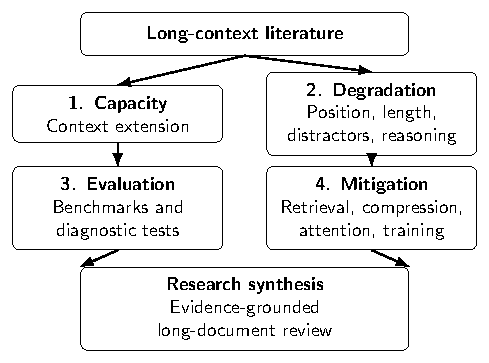
\includegraphics[width=.82\linewidth]{Figures/taxonomy.pdf}
\caption{Taxonomy of the reviewed literature and its relevance to long-document research synthesis.}
\Description{A taxonomy dividing the literature into capacity, degradation, evaluation, and mitigation, leading to evidence-grounded research synthesis.}
\label{fig:taxonomy}
\end{figure}
\clearpage

\section{Thematic Literature Review}\label{sec:literature}
\subsection{Context Extension and the Difference Between Capacity and Effective Use}\label{sec:capacity}
A first research direction attempts to increase the length of sequences that models can process. Train-Short-Test-Long work shows that attention design can improve length extrapolation, while positional interpolation provides another route for scaling a pretrained model to longer contexts \cite{press2022train,chen2023extending}. These methods address a real systems constraint: the model must first be able to represent and process long sequences.

However, later evaluation literature shows that capacity and effective use are different. LongBench evaluates multiple long-context tasks, and Long-context LLMs Struggle with Long In-context Learning shows that performance becomes difficult when tasks require many demonstrations and large label spaces \cite{bai2024longbench,li2025longcontexticl}. Thus, context extension is necessary for some applications but is not sufficient for dependable research synthesis.

\subsection{Empirical Context-Window Degradation}\label{sec:degradation}
The strongest empirical evidence comes from position-sensitive and length-sensitive evaluations. Lost in the Middle reports a U-shaped pattern in which relevant information near the beginning or end of a long input can be used more successfully than information placed in the middle \cite{liu2024lost}. This finding is important because a research document is not naturally organized to place decisive evidence at a privileged position.

More recent work strengthens the distinction between retrieval and downstream use. Context Length Alone Hurts LLM Performance Despite Perfect Retrieval reports substantial degradation even when relevant information is retrieved and remains within the claimed context window \cite{du2025contextlength}. Positional Biases Shift as Inputs Approach Context Window Limits further indicates that positional effects change as inputs approach the model's limit \cite{veseli2025positional}. Together, these studies suggest that context degradation is not simply a search problem: even correctly retrieved evidence may be difficult to use once it is embedded in a sufficiently large context.

\subsection{Long-Context Reasoning and Multi-Document Synthesis}\label{sec:reasoning}
Research synthesis requires more than locating a single answer. Long-context reasoning benchmarks distribute information through extended contexts and require models to combine multiple pieces of evidence. LongBench broadens evaluation across single-document QA, multi-document QA, summarization, few-shot learning, synthetic tasks, and code completion \cite{bai2024longbench}. Long-context in-context learning studies similarly show that increasing demonstrations and label complexity can expose reasoning limitations \cite{li2025longcontexticl}.

These results point toward a deeper failure mode: a model may retrieve individual facts but still fail to combine them into a multi-step conclusion. NoLiMa makes this distinction especially clear by reducing lexical overlap between the question and relevant evidence, requiring models to infer latent associations rather than exploit literal matches \cite{modarressi2025nolima}. This is closer to research synthesis, where a conclusion may depend on evidence expressed using different terminology across papers.

\subsection{Evaluation and Benchmark Development}\label{sec:evaluation}
A major trend is the development of increasingly diagnostic benchmarks. LongBench established a broad bilingual and multitask framework; NoLiMa moves beyond literal matching; and recent work studies context-length effects even under controlled retrieval conditions \cite{bai2024longbench,modarressi2025nolima,du2025contextlength}. This progression reveals an evaluation problem: a model may perform well on a synthetic retrieval task while failing on multi-document reasoning, or appear robust until the input approaches its advertised maximum.

Effective context size should therefore be reported together with task type, evidence position, distractor density, reasoning depth, and document structure. These dimensions connect directly to the benchmark taxonomy in Figure~\ref{fig:taxonomy} and the research-synthesis workflow in Figure~\ref{fig:conceptual-framework}.

\subsection{Mitigation Through Retrieval, Efficient Attention, Training, and Alignment}\label{sec:mitigation}
Retrieval-based approaches reduce irrelevant material presented to the model. This can lower distraction and computational cost, but retrieval can also introduce failure when the wrong evidence is selected or when several pieces of evidence must be jointly reasoned over.

Efficient attention methods target the computational cost of long-context inference. Long-context training and alignment instead aim to teach models to operate more effectively at larger lengths. LOGO applies preference optimization to long-context alignment, while Untie the Knots uses data augmentation during continued pretraining to improve long-context capability \cite{tang2025logo,tian2025untie}. Scaling Granite Code Models illustrates a related training strategy for effective 128K context in code models \cite{stallone2024granite}. These approaches address different layers of the problem, so their value should be interpreted together with evaluation results rather than as a single universal solution.

\subsection{Implications for Long-Document Research Synthesis}\label{sec:implications}
Research synthesis is a particularly demanding long-context application because relevant evidence is rarely a single contiguous passage. A review may require locating the research question in one paper, methodology in another, limitations in a third, and conflicting findings in several others. The model must then construct a conclusion while preserving distinctions between observations, interpretations, and claims.

The distinction between retrieval and synthesis is especially important. Lost in the Middle shows that relevant information can become harder to use depending on position, while length-sensitive studies show that performance can decline even when retrieval is controlled \cite{liu2024lost,du2025contextlength}. This implies that a research-review system should not be evaluated only on whether it can locate a passage; it should also be tested on whether it can connect multiple passages into a correct, source-grounded argument.

For practical literature review, this supports a layered design: discovery identifies candidate papers, retrieval selects evidence, reasoning compares methods and findings, and synthesis produces the final review. Long context may be used selectively rather than indiscriminately. The distinction between nominal capacity and effective use is therefore central to the comparison in Section~\ref{sec:comparison}.

\section{Taxonomy and Comparison of Existing Approaches}\label{sec:comparison}
Table~\ref{tab:approaches} compares five approach families. The taxonomy distinguishes whether an approach primarily changes capacity, evidence selection, model computation, model training, or evaluation. This separation prevents very different interventions from being compared as though they solved the same problem.

\begin{table*}[t]
\centering
\caption{Comparison of Existing Approaches for Long-Context Use}
\label{tab:approaches}
\small
\begin{tabularx}{\textwidth}{>{\raggedright\arraybackslash}p{.18\textwidth} X X X}
\toprule
\textbf{Approach} & \textbf{Strength} & \textbf{Main limitation} & \textbf{Implication for research synthesis}\\
\midrule
Context extension / positional methods & Increase nominal usable sequence length and allow models to process longer inputs. & Longer capacity does not ensure uniform use of information. & Necessary foundation, but must be paired with effective-use evaluation.\\
Retrieval / context reduction & Removes irrelevant material and can reduce distraction and computation. & Can miss evidence or break cross-document dependencies. & Useful when documents are numerous, but retrieval quality and evidence coverage must be evaluated.\\
Long-context training / alignment & Improves adaptation to long sequences and task behavior. & Training cost and generalization remain concerns. & Promising for domain-specific synthesis systems when evaluated beyond a single benchmark.\\
Efficient / sparse attention & Reduces computational cost for large contexts. & Efficiency gains do not automatically remove semantic degradation. & Important for deployable long-document systems, but efficiency must be separated from reliability.\\
Benchmarking / inference-time correction & Makes hidden failure modes measurable and can sometimes reduce them. & Benchmarks may still simplify real research workflows. & Necessary for deciding whether a claimed context window is practically useful.\\
\bottomrule
\end{tabularx}
\end{table*}

As shown in Table~\ref{tab:approaches}, the approaches address different parts of the long-context problem rather than a single common failure mode. The evidence on degradation discussed in Section~\ref{sec:degradation} provides the reliability context in which these approaches should be interpreted.

\subsection{Context Extension Versus Effective Context Use}\label{sec:context-comparison}
Context-extension methods solve a capacity problem, whereas degradation studies expose a reliability problem. Positional Interpolation and ALiBi demonstrate that models can be adapted to longer sequences \cite{press2022train,chen2023extending}. Scaling Granite Code Models similarly demonstrates an approach to effective 128K context for code tasks \cite{stallone2024granite}. These results are important because without adequate capacity, a model cannot receive a large research corpus.

However, the evaluation literature indicates that maximum supported length is not equivalent to effective context size. Lost in the Middle, NoLiMa, and Context Length Alone Hurts LLM Performance Despite Perfect Retrieval all show, in different ways, that long input can reduce performance \cite{liu2024lost,modarressi2025nolima,du2025contextlength}. A model may therefore advertise a large window while delivering materially different quality at different fractions of that window. Future reporting should include performance curves across context lengths rather than one maximum-token number.

\subsection{Retrieval, Compression, and Full-Context Reasoning}\label{sec:retrieval}
Retrieval and compression are attractive because they reduce the amount of material the model must process. However, aggressive reduction can remove evidence needed for synthesis. This creates a central trade-off: reducing context can lower distraction, but retaining context can preserve cross-document dependencies.

A research-review workflow should therefore treat retrieval as an adaptive operation rather than a universal replacement for long context. For a question requiring one specific fact, retrieval can be sufficient. For a question requiring comparison across several papers, hierarchical retrieval may be safer: first retrieve relevant documents, then relevant sections, then enough surrounding evidence for cross-document reasoning. This design aligns better with the structure of academic literature than either blindly passing every document or reducing every task to a single retrieved passage.

\section{Research Trends and Developments}\label{sec:trends}
The literature is moving from nominal context length toward effective context size; from single-fact retrieval toward distributed reasoning; from literal matching toward semantic understanding; and from isolated architecture changes toward hybrid systems. Evaluation is also becoming more diagnostic by varying evidence position, context utilization, distractor density, and reasoning complexity.

\subsection{From Benchmark Scores to Application Reliability}\label{sec:application}
A single benchmark score can hide a failure mode that becomes severe in actual research use. For long-document synthesis, future benchmarks should combine the dimensions that the current literature often tests separately: document count, context length, evidence position, distractor density, number of reasoning steps, and source attribution. A model should receive credit only when it reaches a correct conclusion for the right evidence, not merely when its final answer happens to match a reference answer.

\section{Challenges and Limitations}\label{sec:limitations}
The evidence base has several limitations. Many studies use controlled or synthetic tasks because these make failure modes measurable. That is scientifically useful, but real literature reviews contain heterogeneous documents, tables, references, equations, inconsistent terminology, and conflicting claims. Papers also differ in model generations, context sizes, and evaluation protocols, making direct numerical comparison difficult.

Another limitation is publication and discovery bias. The four discovery tools do not expose identical scholarly corpora, and papers that are highly connected or recently published may be surfaced more easily. The final 20-paper set is therefore an evidence base for thematic analysis, not a systematic review in the strict PRISMA sense. Human screening remains necessary to check relevance, bibliographic accuracy, and whether a paper's findings actually support a claim in the final review.

\section{Research Gaps}\label{sec:gaps}
The review identifies six gaps that are particularly relevant to long-document research synthesis:
\begin{enumerate}
\item No single standard yet measures effective context size across realistic research-synthesis tasks.
\item More evaluation is needed for multi-document synthesis where evidence is distributed across documents and some sources are intentionally distracting.
\item Long-context evaluation should jointly measure retrieval, reasoning, synthesis quality, and source attribution rather than treating them as separate capabilities.
\item Research is needed on how document ordering, section structure, tables, references, and heterogeneous file formats affect degradation.
\item Human-centered evaluation is needed to determine whether benchmark improvements translate into better academic or professional literature reviews.
\item Mitigation methods should be compared under comparable compute and accuracy constraints so that context extension, retrieval, and compression can be evaluated fairly.
\end{enumerate}

\subsection{Specific Research Gaps for Long-Document Research Synthesis}\label{sec:specific-gaps}
First, there is a gap between long-context benchmarks and actual literature-review workflows. Many benchmarks test controlled retrieval or reasoning; fewer require a model to compare competing studies, preserve methodological differences, resolve contradictory findings, and produce evidence-grounded synthesis.

Second, source attribution deserves stronger treatment. A research assistant should identify which document and passage support each important claim. Long-context degradation could cause a model to produce a plausible synthesis while silently ignoring a critical limitation or attributing a result to the wrong paper.

Third, context structure should be treated as an experimental variable. Scientific documents have headings, abstracts, tables, references, and repeated terminology. Reordering or compressing such structure may change model behavior. Evaluating structured scientific documents rather than generic passages would make results more relevant to academic research.

Finally, the field needs clearer decision rules for choosing between full-context inference, retrieval, compression, and hierarchical summarization. A future literature-review assistant should estimate task difficulty and evidence distribution before deciding how much context to expose to the model.

\section{Future Research Directions}\label{sec:future}
\begin{itemize}
\item Develop research-review benchmarks with realistic collections of papers, explicit evidence chains, and controlled distractors.
\item Report effective-context curves instead of only maximum token limits.
\item Combine retrieval with long-context reasoning and test when retrieval helps versus when it removes useful cross-document dependencies.
\item Develop position-robust and structure-aware training methods so that important evidence can be used regardless of where it appears.
\item Evaluate source attribution and claim-evidence consistency as first-class long-context metrics.
\item Study adaptive inference policies that choose between full context, retrieval, compression, and hierarchical summarization based on task difficulty.
\end{itemize}

\section{Conclusion}\label{sec:conclusion}
The literature reviewed here indicates that context-window degradation is a practical reliability problem rather than merely a hardware or token-limit problem. Models may accept long inputs while failing to use information uniformly, particularly when evidence is positioned in the middle, when contexts approach their limits, or when reasoning requires multiple distributed facts. Long-context benchmarks have made these failures more visible, while context extension, retrieval, efficient attention, training, and alignment provide partial mitigation strategies.

For long-document research synthesis, the strongest conclusion is that no single metric or technique is sufficient. A credible workflow should combine broad literature discovery, citation-linked exploration, structured comparison, and human verification. The final system should be evaluated on realistic multi-document reasoning, evidence integration, and source fidelity, not merely on whether it can ingest a large context window.

\section*{Acknowledgments}
This review preserves the assigned research topic and evidence base while reorganizing the literature for ACM Computing Surveys-style presentation.

\nocite{*}
\bibliographystyle{ACM-Reference-Format}
\bibliography{references}

\end{document}
